\section{Lyapunov Stability Analysis on Euclidean Spaces}

\begin{frame}[standout, plain, noframenumbering]
    Lyapunov Stability Analysis on Euclidean Spaces

    % \medskip

    % \footnotesize
    % Sam Greydanus \quad Misko Dzamba \quad Jason Yosinski
\end{frame}

\begingroup
\small

\begin{frame}
    \frametitle{Autonomous Systems}

    Consider the autonomous system 
    \begin{equation}
        \dot{x} = f(x)
        \label{eq:autonomous}
    \end{equation}
    where $f: D \subseteq \mathbb{R}^n \rightarrow \mathbb{R}^n$ is a locally
    Lipschitz map, with an equilibrium point at $x = 0$.

    \begin{definition}
        The equilibrium point $x=0$ of the system~\eqref{eq:autonomous} is
        \begin{itemize}
            \item \textit{stable} if, $\forall \varepsilon > 0$, $\exists \delta
            = \delta(\varepsilon) > 0$ such that 
            \[
                \norm{x(0)}{} < \delta \; \Rightarrow \; \norm{x(t)}{} < 
                \epsilon, \; \; \forall t \geq 0.
            \]
            \item \textit{unstable} if it is not stable.
            \item \textit{asymptotically stable} if it is stable and $\delta$
            can be chosen s.t.
            \[ \norm{x(0)}{} < \delta \; \Rightarrow \; \lim_{t \to \infty} x(t)
            = 0. \]
        \end{itemize}
    \end{definition}
\end{frame}


\begin{frame}
    \frametitle{Example -- Pendulum}

    The pendulum equation
    \begin{align*}
        \dot{x}_1 &= x_2 \\
        \dot{x}_2 &= -a \sin{x_1} - b x_2
    \end{align*}
    has two equilibrium points at ($x_1 = 0$, $x_2 = 0$) and ($x_1 = \pi$, $x_2
    = 0$).
    %
    \begin{itemize}
        \item If $b=0$, trajectories in the nbhd. of the first equilibrium are 
        closed orbits.
        \item By starting sufficiently close to the eq. point, trajectories are 
        guaranteed to stay within any specified ball.
        \item The point is not asymptotically stable since trajectories don't
        tend to the eq. point.
        \item If $b > 0$, the origin becomes asymptotically stable.
        \item The second eq. point is a saddle point: the $\varepsilon-\delta$
        requirement cannot be satisfied (for every $\varepsilon > 0$ there
        exists a trajectory that will leave the ball $B_\varepsilon$ even if
        $x(0)$ is arbitrarily close to $(\pi, 0)$).
    \end{itemize}
\end{frame}


\begin{frame}
    \frametitle{Lyapunov Stability Theorem}

    \begin{theorem}
        Let $x=0 \in D$ be an equilibrium point for~\eqref{eq:autonomous}. Let
        $V: D \rightarrow \mathbb{R}$ be a continuously differentiable function
        such that
        \begin{align*}
            V(0) = 0 \; &\text{ and } \; V(x) > 0 \text{ in } D - \{0\}, \\
            &\dot{V}(x) \leq 0 \text{ in } D.
        \end{align*}
        Then, $x=0$ is stable. Moreover, if
        \[ \dot{V}(x) < 0 \text{ in } D - \{0\} \] then $x=0$ is asymptotically
        stable.
    \end{theorem}
\end{frame}


\begin{frame}
    \frametitle{Lyapunov Stability Theorem}

    \begin{proof}[Proof of stability]
        Given $\varepsilon > 0$, choose $0 < r \leq \varepsilon$ such that $B_r
        \subseteq D$. Let $\alpha = \min_{\norm{x}{}=r} V(x)$. Then, $\alpha >
        0$. Take $0 < \beta < \alpha$ and consider $\mc{M}_\beta = V^{-1}((0,
        \beta])$.

        \underline{Claim}: $\mc{M}_\beta \subseteq \accentset{\circ}{B}_r$.
        Argue ad absurdum. Suppose $\mc{M}_\beta \cap \accentset{\circ}{B}_r
        \neq \mc{M}_\beta$. Then $\exists p \in \mc{M}_\beta \cap \partial B_r$.
        Note, $V(p) \geq \alpha > \beta$, but $V(\mc{M}_\beta) \subseteq
        [0,\beta]$.

        The set $\mc{M}_\beta$ is invariant since \[ \dot{V}(x(t)) \leq 0 \;
        \Rightarrow \; V(x(t)) \leq V(x(0)) \leq \beta, \; \forall t \geq 0. \]

        Because $\mc{M}_\beta$ is compact (closed and bounded), we conclude that
        the ODE~\eqref{eq:autonomous} has a unique solution $\forall t \geq 0$
        whenever $x(0) \in \mc{M}_\beta$. Since $V$ is continuous and $V(0) =
        0$, $\exists \delta > 0$ such that \[ \norm{x}{} \leq \delta \;
        \Rightarrow \; V(x) < \beta. \]
    \end{proof}
\end{frame}

\begin{frame}
    \frametitle{Lyapunov Stability Theorem}

    \begin{proof}[Proof of stability (cont'd)]
        Then, \[ B_\delta \subseteq \mc{M}_\beta \subseteq B_r \] and 
        \[ x(0) \in B_\delta \; \Rightarrow \; x(0) \in \mc{M}_\beta \;
        \Rightarrow \; x(t) \in \mc{M}_\beta \; \Rightarrow \; x(t) \in B_r, \]
        proving stability.
    \end{proof}

    \begin{figure}[bth]
        \centering
        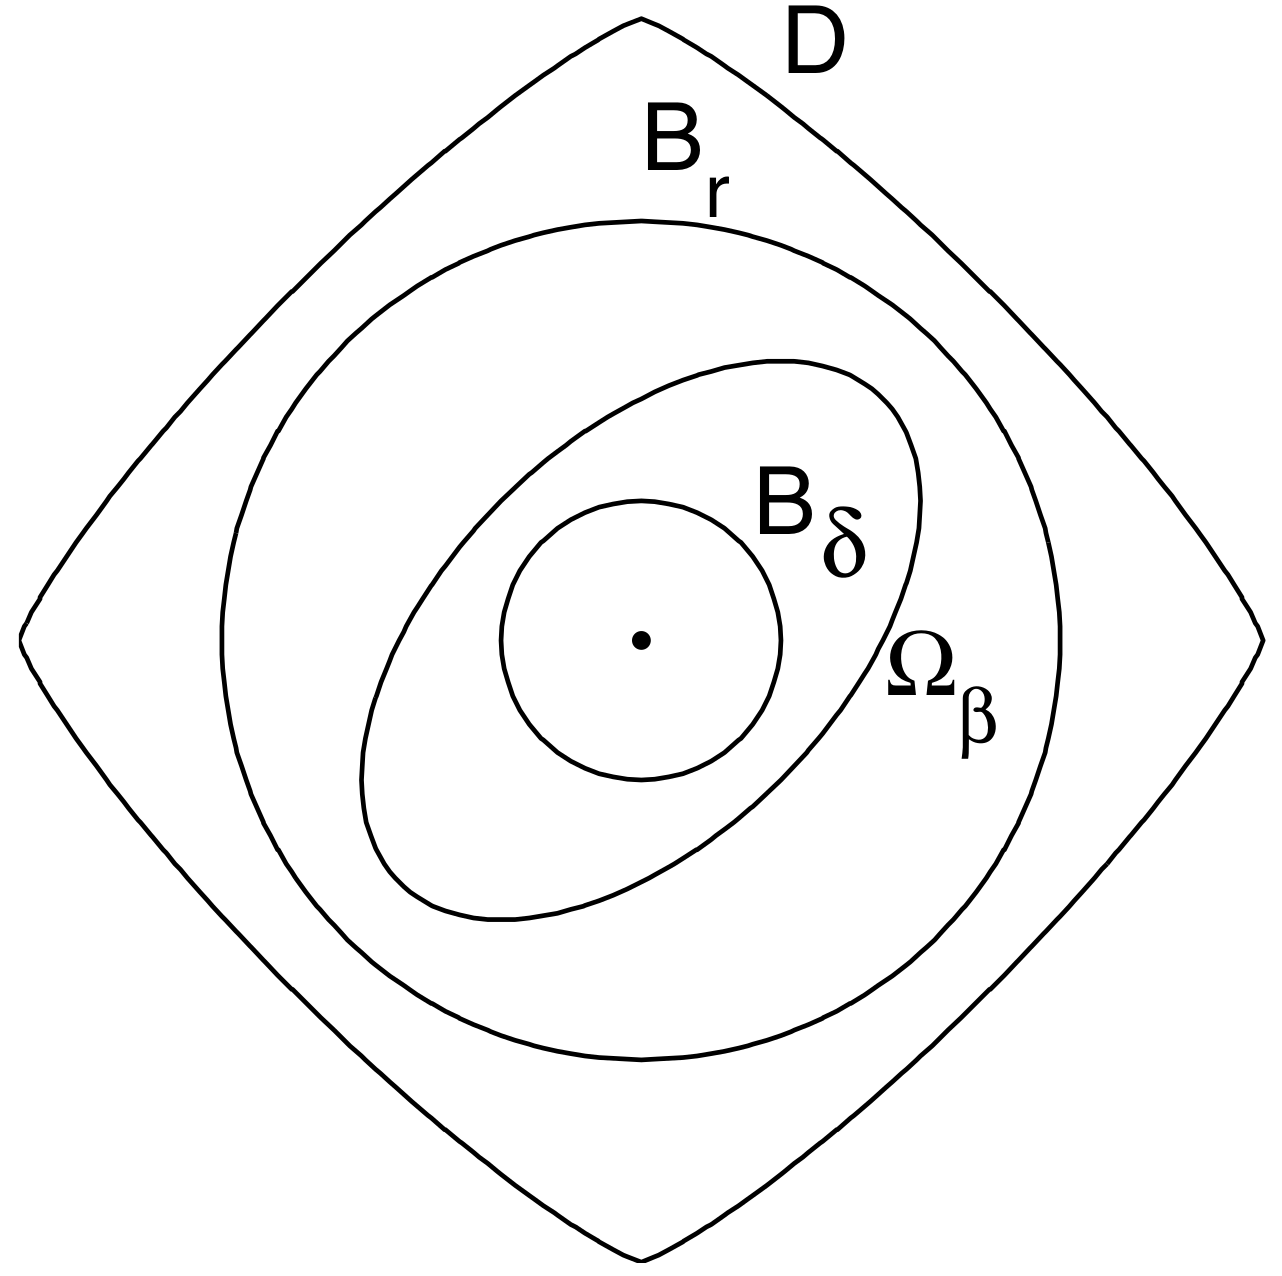
\includegraphics[width=0.35\textwidth]{figures/lyap_geometry.png} 
        \caption{\footnotesize Geometric representation of Lyapunov stability.}
    \end{figure}
\end{frame}

\begin{frame}
    \frametitle{Lyapunov Stability Theorem}

    \begin{proof}[Proof of asymptotic stability]
        Now assume $\dot{V}(x) < 0$ in $D - \{0\}$. We want to show that $x(t)
        \xrightarrow{t \to \infty} 0$; i.e., $\forall a > 0$, $\exists T > 0$, 
        s.t. $\norm{x(t)}{} < a, \forall t > T$.

        We know that $\forall a > 0$, we can choose $b > 0$ s.t. $\mc{M}_b
        \subseteq B_a$. Therefore, it is sufficient to show that $V(x(t))
        \xrightarrow{t \to \infty} 0$. Since $V$ is monotonically decreasing and
        bounded from below by zero, \[ V(x(t)) \xrightarrow{t \to \infty} c \geq
        0. \]

        \underline{Claim}: $c = 0$. Argue ad absurdum. Suppose $c > 0$. By
        continuity of $V$, $\exists d > 0$ s.t. $B_d \subseteq \mc{M}_c$. The
        limit $V(x(t)) \rightarrow c > 0$ implies that $x(t) \notin B_d, \forall
        t \geq 0$. Define $\max_{d \leq \norm{x}{} \leq r} \dot{V}(x) =: -\gamma
        < 0$. It follows that 
        \[
        V(x(t)) = V(x(0)) + \int_0^t \dot{V}(x(\tau)) \dd \tau \leq V(x(0)) - \gamma t.
        \]
        The RHS will eventually become negative: contradiction ($c > 0$).
    \end{proof}
\end{frame}


\begin{frame}
    \frametitle{Lyapunov Stability: Intuition}
    \begin{figure}[bth]
        \centering
        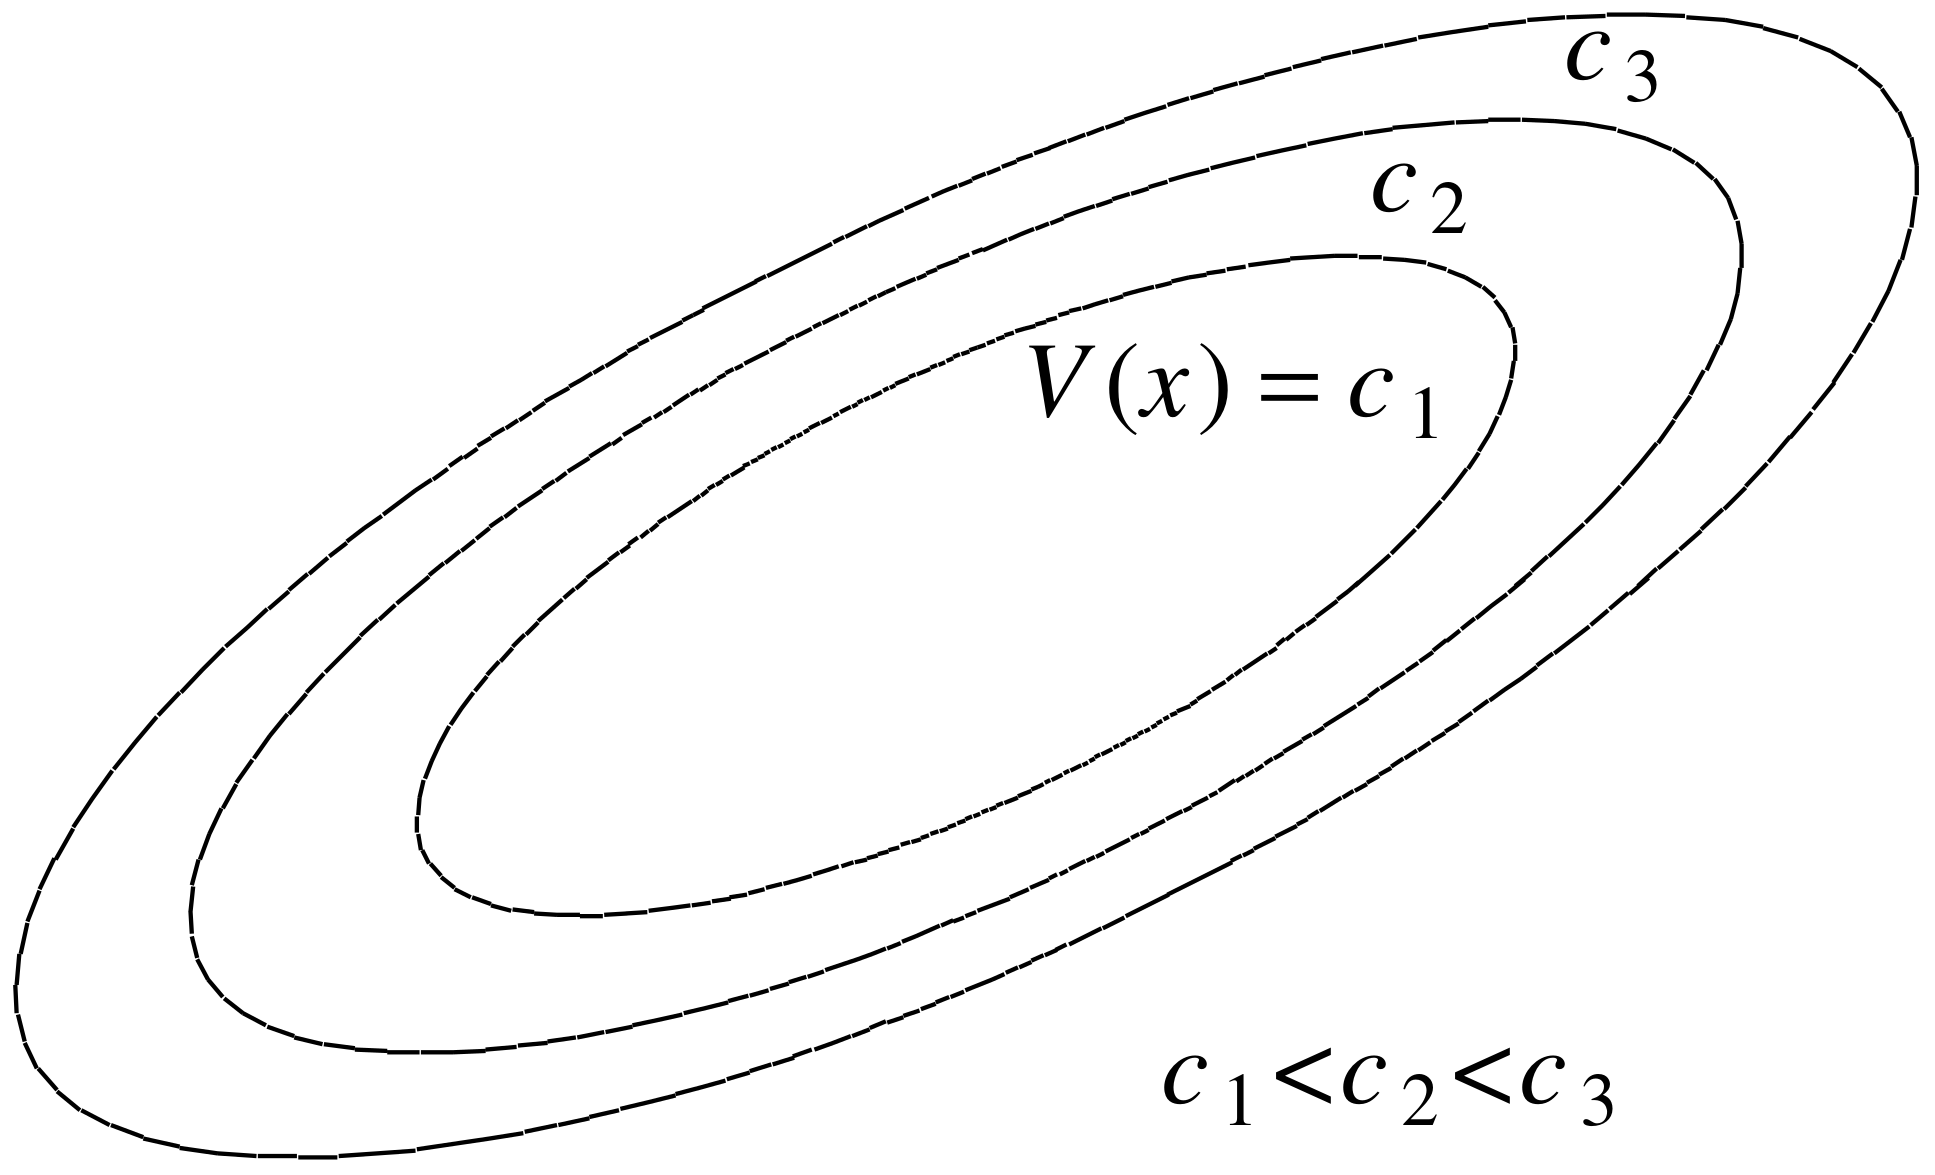
\includegraphics[width=0.35\textwidth]{figures/lyap_level_sets.png} 
        % \caption{\footnotesize Geometric representation of Lyapunov stability.}
    \end{figure}

    \begin{itemize}
        \item A continuously differentiable function $V$, satisfying the
        theorem's conditions is called a \textsc{Lyapunov function}.
        \item When $\dot{V} < 0$, the trajectory moves from level set
        $\mc{M}_{c_3} = V^{-1}(c_3)$ to an inner level set $\mc_{M}_{c_2} =
        V^{-1}(c_2)$ with a smaller $c$.
        \item $V^{-1}(c) \xrightarrow{c \downarrow 0} 0$. Hence the trajectory
        approaches the origin.
        \item If we only knew that $\dot{V} \leq 0$, we cannot be sure that the
        trajectory $x(t) \xrightarrow{t \to \infty} 0$,\footnotemark but we can
        conclude that the origin is stable.
    \end{itemize}

    \footnotetext{See, however, Krasovskii-LaSalle's theorem.}
\end{frame}


\begin{frame}
    \frametitle{Example: Undamped pendulum}

    \begin{columns}
        \begin{column}{0.5\textwidth}
            \begin{align*}
                \dot{x}_1 &= x_2, \\
                \dot{x}_2 &= -a \sin{x_1}.
            \end{align*}
        \end{column}
        \begin{column}{0.5\textwidth}
            \underline{Lyapunov function candidate}\\[0.75ex]
            $ V(x) = a(1 - \cos{x_1}) + \frac{1}{2}x_2^2. $
        \end{column}
    \end{columns}
    \begin{block}{Analysis}
        Clearly, $V(0) = 0$ and $V(x) > 0$ if $x \neq (2 k \pi, 0)$. Compute the 
        Lie derivative of $V$ along $f$:
        \[ \dot{V}(x) = \mc{L}_fV(x) = a x_2 \sin{x_1} - a x_2 \sin{x_1} = 0. \]
        Thus, the origin is stable. Since $\dot{V}(x) \equiv 0$, we conclude
        that the origin is not asymptotically stable as solutions starting on
        the level set $\mc{M}_c$ remain in that set.
    \end{block}
\end{frame}


\begin{frame}
    \frametitle{Example: Damped pendulum}

    \begin{columns}
        \begin{column}{0.5\textwidth}
            \begin{align*}
                \dot{x}_1 &= x_2, \\
                \dot{x}_2 &= -a \sin{x_1} - bx_2.
            \end{align*}
        \end{column}
        \begin{column}{0.5\textwidth}
            \begin{center}
                \underline{Lyapunov function candidate}
            \end{center}
            \vspace{-5mm}
            \begin{align*}
                V(x) &= a(1 - \cos{x_1}) + \frac{1}{2}x^\top P x, \\
                P &= P^\top > 0.
            \end{align*}
        \end{column}
    \end{columns}
    The Lie derivative $\dot{V}(x)$ is given by 
    \begin{equation*}
        \dot{V}(x) = a(1-p_{22})x_2 \sin{x_1} - ap_{12}x_1 \sin{x_1} + (p_{11} - p_{12}b)x_1x_2 + (p_{12}-p_{22}b)x_2^2.
    \end{equation*}

    \begin{itemize}
        \item Take $p_{22} = 1$ and $p_{11} = bp_{12}$.
        \item We must choose $0 < p_{12} < b$ for $V$ to be positive definite. 
        \item Choose $p_{12} = \frac{b}{2}$.
    \end{itemize}

     \begin{equation*}
        \dot{V}(x) = -\frac{1}{2}a b x_1 \sin{x_1} - \frac{1}{2}bx_2^2.
     \end{equation*}

     This is negative definite for any $0 < \abs{x_1} < \pi$.
\end{frame}


\begin{frame}
    \frametitle{Region of Attraction}

    \begin{definition}[Region of Attraction]
        The \textsc{region of attraction} is defined as the set of all points
        $x$ such that $\phi(t; x)$ is defined for all $t \geq 0$ and $\lim_{t
        \to \infty} \phi(t; x) = 0$.
    \end{definition}
    \begin{itemize}
        \item Finding the exact RoA is usually difficult.
        \item Lyapunov fcns. can be used to estimate (inner approx.) the RoA.
        \item From the proof of the Lyapunov stability theorem, if there is a
        Lyapunov fcn. that satisfies asymptotic stability and if $\mc{M}_c$ is
        bounded and contained in $D$, then $\mc{M}_c$ is (positively) invariant.
        \item The estimate $\mc{M}_c$ of the RoA may be conservative (inner
        approximation).
        \item \textsc{Question}: Under what conditions is the RoA the whole space?
        \begin{itemize}
            \item If so, the origin is said to be \textit{globally asymptotically stable}.
            \item The conditions of the Lyapunov theorem must clearly hold for
            $D = \mathbb{R}^n$. But is this sufficient?
        \end{itemize}
    \end{itemize}
\end{frame}


\begin{frame}
    \frametitle{Region of Attraction}
    \only<1>{
    \begin{figure}[bth]
        \centering
        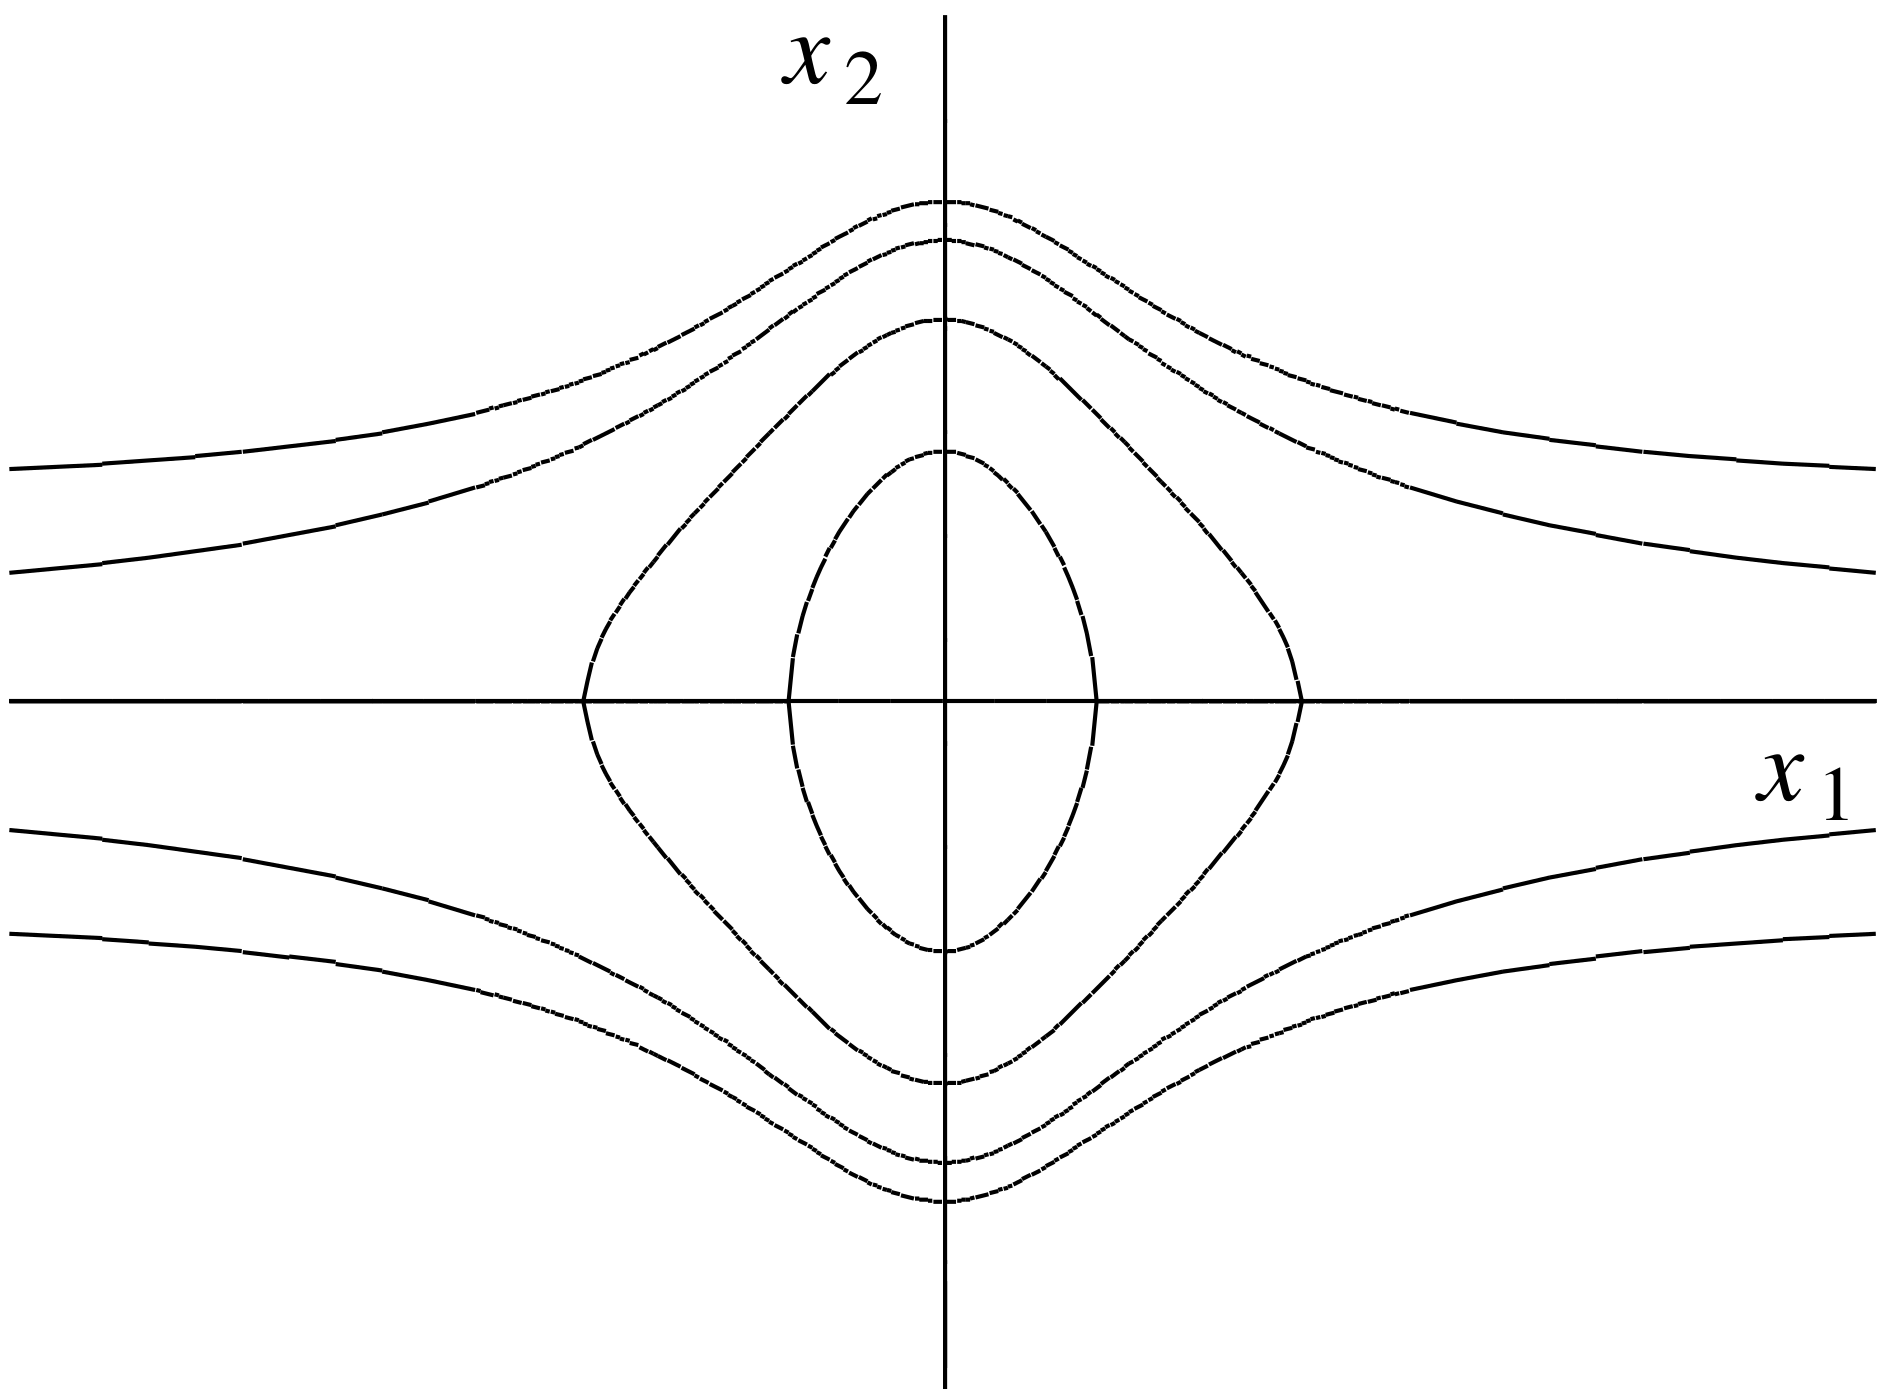
\includegraphics[width=0.35\textwidth]{figures/lyap_surfaces.png} 
        % \caption{\footnotesize Geometric representation of Lyapunov stability.}
    \end{figure}
    }
    For $\mc{M}_c$ to be bounded ($\mc{M}_c \subseteq \accentset{\circ}{B}_r$,
    for some $r \geq 0$), $c < \inf_{\norm{x}{} \geq r}V(x)$. If \[ l = \lim_{r
    \to \infty} \inf_{\norm{x}{} \geq r} V(x) < \infty \] then $\mc{M}_c$ will be bounded only if $c < l$.
    Consider (see figure) \[ V(x) =
    \frac{x_1^2}{1 + x_1^2} + x_2^2. \] In this example, 
    \[ l = \lim_{r \to \infty} \min_{\norm{x}{}=r} V(x) = 1. \] 

    \onslide<2->{
    An extra
    condition that ensures that $\mc{M}_c$ is bounded for all $c > 0$ is \[ V(x)
    \to \infty \; \text{ as } \; \norm{x}{} \to \infty. \]
    }
\end{frame}

\begin{frame}
    \frametitle{Region of Attraction}

    \begin{theorem}[Global Asymptotic Stability]
        Let $V: \mathbb{R}^n \rightarrow \mathbb{R}$ be a continuously
        differentiable function and the conditions of the Lyapunov stability
        theorem hold (\textit{asymptotic}). If, in addition, \[ \norm{x}{} \to
        \infty \; \Rightarrow \; V(x) \to \infty \] then $x=0$ is
        \textit{globally asymptotically stable}.
    \end{theorem}
    
    \begin{rem}
        For $x=0$ to be GAS, it must be the unique equilibrium point of the
        system (why?).
    \end{rem}
\end{frame}


\begin{frame}
    \frametitle{Chetaev's Instability Theorem}

    \begin{theorem}
        Let $V: D \rightarrow \mathbb{R}$ be a continuously differentiable
        function such that $V(0) = 0$ and $V(x_0) > 0$ for some $x_0$ with
        arbitrarily small $\norm{x_0}{}$. Let\\[0.5ex] \hspace{35mm} $U := \{ x
        \in B_r: V(x) > 0\}$\\[0.5ex] and suppose that $\dot{V}(U) > 0$. Then,
        $x=0$ is unstable.
    \end{theorem}

    \begin{proof}
        $x_0 \in \accentset{\circ}{U}$ and $V(x_0) = a > 0$. The trajectory
        $x(t)$ starting at $x(0) = x_0$ must leave $U$. Indeed, as long as $x(t)
        \in U$, $V(x(t)) \geq a$, since $\dot{V}(U) > 0$. Let $\min 
        \{\dot{V}(x): x \in U \text{ and } V(x) \geq a \} := \gamma > 0$.  Then, 
        \[ V(x(t)) = V(x_0) + \int_0^t \dot{V}(x(s)) \dd s \geq a + \int_0^t
        \gamma \dd s = a + \gamma t. \] Hence, $x(t)$ will leave $U$ because
        $V(x)$ is bounded on $U$. Now, $x(t)$ cannot leave $U$ through $V(x) =
        0$ since $V(x(t)) \geq a$. Hence it must leave $U$ through the sphere
        $\mathbb{S}_r$. Note: $\norm{x_0}{}$ was arbitrarily small.
    \end{proof}
\end{frame}

\endgroup